% ./dc -meta ./meta -preamble <path_to_latex_preamble> <path_to_tex>

% ./dc -meta ./meta -preamble latex_preamble/preamble.tex ./05_Undecidability/Chapter_05_Undecidability.tex

\chapter{Undecidable Languages}
\label{chapter:Undecidable-Languages}

\begin{preamble}
In this chapter, we formally prove that almost all languages are undecidable using the countability and uncountability concepts from a previous chapter. We also present (with proofs) several explicit examples of undecidable languages. By the Church-Turing Thesis, these results highlight the inherint limitations of computation.

An important tool in showing that a language is undecidable is the concept of a \emph{reduction}. We present this technique in this chapter. Reductions play an extremely important role in computer science. In fact, we will revisit them in a future chapter (in the context of the famous $\mathsf{P}$ vs $\mathsf{NP}$ problem.)

Our goal in this chapter is for you to get comfortable with undecidability proofs and the concept of reductions, as they are at the core of the study of computation.
\end{preamble}



\section{Existence of Undecidable Languages}

\begin{flex}
\begin{proposition}[The set of Turing machines is countable]  \label{proposition:The-set-of-Turing-machines-is-countable}
Fix some input alphabet and tape alphabet. The set of all Turing machines $\{M : M \text{ is a TM}\}$ is countable.
\end{proposition}

\begin{proof}
Let $T = \{M : M \text{ is a TM}\}$. We want to show that $T$ is countable. We will do so by using the CS method of showing a set is countable. 

Given any Turing machine, there is a way to encode it with a finite length string because each component of the $7$-tuple has a finite description. In particular, the mapping $M \mapsto \langle M \rangle$, where $\langle M \rangle \in \Sigma^*$, for some finite alphabet $\Sigma$, is an injective map (two distinct Turing machines cannot have the same encoding). Therefore $|T| \leq |\Sigma^*|$. And since $\Sigma^*$ is countable (Proposition~\ref{proposition:Sigma-is-countable}), i.e., $|\Sigma^*| \leq |\N|$, the result follows.
\end{proof}
\end{flex}


\begin{flex}
\begin{theorem}[Almost all languages are undecidable] \label{theorem:Almost-all-languages-are-undecidable}
Fix some alphabet $\Sigma$. There are languages $L \subseteq \Sigma^*$ that are \textbf{not} decidable.
\end{theorem}

\begin{proof}
To prove the result, we simply observe that the set of all languages is uncountable whereas the set of decidable languages is countable. First, consider the set of all languages. Since a language $L$ is defined to be a subset of $\Sigma^*$, the set of all languages is $\calP(\Sigma^*)$. By Corollary~\ref{corollary:The-set-of-languages-is-uncountable}, we know that this set is uncountable. Now consider the set of all decidable languages, which we'll denote by $D$. Let $T$ be the set of all TMs. By Proposition~\ref{proposition:The-set-of-Turing-machines-is-countable}, we know that $T$ is countable. Furthermore, the mapping $M \mapsto L(M)$ can be viewed as a surjection from $T$ to $D$ (if $M$ is not a decider, just map it to $\emptyset$). So $|D| \leq |T|$. Since $T$ is countable, this shows $D$ is countable and completes the proof.
\end{proof}
\end{flex}


\begin{note}[Constructive vs non-constructive proofs] \label{note:Constructive-vs-non-constructive-proofs}
The argument above is called \emph{non-constructive} because it does not present an explicit undecidable language. A \emph{constructive} argument would prove the undecidability of an explicit language. We present such an argument below (Theorem~\ref{theorem:Turings-Theorem}). 
\end{note}






\section{Examples of Undecidable Languages}


\begin{definition}[Halting problem] \label{definition:Halting-problem} 
The \defn{halting problem} is defined as the decision problem corresponding to the language
$$
\text{HALTS} = \{\bkt{M,x} : \text{$M$ is a TM which halts on input $x$} \}.
$$
\end{definition}


\begin{flex}
\begin{theorem}[Turing's Theorem] \label{theorem:Turings-Theorem}
The language $\mathrm{HALTS}$ is undecidable.
\end{theorem}

\begin{proof}
Our goal is to show that $\text{HALTS}$ is undecidable. The proof is by contradiction, so assume that $\text{HALTS}$ is decidable. By definition, this means that there is a decider TM, call it $M_\text{HALTS}$, that decides $\text{HALTS}$. We construct a new TM, which we'll call $M_\text{TURING}$, that uses $M_\text{HALTS}$ as a subroutine. The description of $M_\text{TURING}$ is as follows:

\begin{center}
\includegraphics[width=0.7\textwidth]{05_Undecidability/media_upload/tm-turing.png}
\end{center}

We get the desired contradiction once we consider what happens when we feed $M_\text{TURING}$ as input to itself, i.e. when we run $M_\text{TURING}(\bkt{M_\text{TURING}})$. 

If $M_\text{HALTS}(\bkt{M_\text{TURING},M_\text{TURING}})$ accepts, then $M_\text{TURING}(\bkt{M_\text{TURING}})$ is supposed to halt by the definition of $M_\text{HALTS}$. However, from the description of $M_\text{TURING}$ above, we see that it goes into an infinite loop. This is a contradiction. The other option is that $M_\text{HALTS}(\bkt{M_\text{TURING},M_\text{TURING}})$ rejects. Then $M_\text{TURING}(\bkt{M_\text{TURING}})$ is supposed to lead to an infinite loop. But from the description of $M_\text{TURING}$ above, we see that it accepts, and therefore halts. This is a contradiction as well.
\end{proof}
\end{flex}


\begin{note}[Diagonalization argument for undecidability] \label{note:Diagonalization-argument-for-undecidability}
The above proof is called a \emph{diagonalization argument} as it is very similar to the proof of Cantor's theorem (Theorem~\ref{theorem:Cantors-Theorem}). As in the proof of Theorem~\ref{theorem:01infty-is-uncountable}, we can present the above proof using a table and flipping its diagonal elements to get the desired contradiction. We do so below.

\emph{Reproof:} The proof is by contradiction, so assume that $\text{HALTS}$ is decidable. By definition, this means that there is a decider TM, call it $M_\text{HALTS}$, that decides $\text{HALTS}$.

The set of all Turing machines is countable (Proposition~\ref{proposition:The-set-of-Turing-machines-is-countable}). Let $M_1, M_2, \ldots$ be a listing of {\bf all} Turing machines in some arbitrary order. We now consider a table in which row $i$ corresponds to $M_i$ and column $i$ corresponds to $\langle M_i \rangle$. At entry corresponding to row $i$ and column $j$, we indicate whether $M_i(\langle M_j \rangle)$ halts or loops forever. If it loops forever, we put a $\infty$ symbol, and if it halts, we put $H$.
\begin{center}
\includegraphics[width=0.5\textwidth]{05_Undecidability/media_upload/tm-diagonal.png}
\end{center}
We now create a new row in this table by taking the diagonal elements of the table and flipping their value (an $\infty$ is flipped to an $H$, and an $H$ is flipped to an $\infty$). Notice that $M_\text{TURING}$ constructed in the previous proof corresponds exactly to this new row we have created. We are able to construct $M_\text{TURING}$ (and therefore the row it corresponds to) because we have a decider for $\text{HALTS}$. The contradiction is reached because on the one hand, $M_\text{TURING}$ should appear as a row in the table since all the Turing machines are listed. On the other hand, the row of $M_\text{TURING}$ differs from every row in the table (by construction, it differs from row $i$ in the $i$'th column), and therefore cannot be in the table.
\end{note}


\begin{definition}[Languages related to encodings of TMs] \label{definition:Languages-related-to-encodings-of-TMs}
We define the following languages:
\begin{itemize}
    \item[] $\text{ACCEPTS} = \{\bkt{M,x} : \text{$M$ is a TM that accepts the input $x$}\}$,
    \item[] $\text{EMPTY} = \{\bkt{M} : \text{$M$ is a TM with $L(M) = \emptyset$} \}$,
    \item[] $\text{EQ} = \{\bkt{M_1,M_2} : \text{$M_1$ and $M_2$ are TMs with $L(M_1) = L(M_2)$} \}$.
\end{itemize}
\end{definition}


\begin{flex}
\begin{theorem}[$\mathrm{ACCEPTS}$ is undecidable] \label{theorem:mathrmACCEPTS-is-undecidable}
The language $\mathrm{ACCEPTS}$ is undecidable.
\end{theorem}

\begin{proof}
We want to show that $\text{ACCEPTS}$ is undecidable. The proof is by contradiction, so assume $\text{ACCEPTS}$ is decidable and let $M_\text{ACCEPTS}$ be a decider for it. We will use this decider to come up with a decider for $\text{HALTS}$. Since $\text{HALTS}$ is undecidable (Theorem~\ref{theorem:Turings-Theorem}), this argument will allow us to reach a contradiction.

Here is our decider for $\text{HALTS}$:

\begin{center}
\includegraphics[width=0.7\textwidth]{05_Undecidability/media_upload/reduction-halts-to-accepts.png}
\end{center}

We now argue that this machine indeed decides $\text{HALTS}$. To do this, we'll show that no matter what input is given to our machine, it always gives the correct answer. 

First let's assume we get any input $\bkt{M,x}$ such that $\bkt{M,x} \in \text{HALTS}$. In this case our machine is supposed to accept. Since $M(x)$ halts, we know that $M(x)$ either ends up in the accepting state, or it ends up in the rejecting state. If it ends up in the accepting state, then $M_\text{ACCEPTS}(\bkt{M,x})$ accepts (on line 1 of our machine's description), and so our program accepts and gives the correct answer on line 2. If on the other hand, $M(x)$ ends up in the rejecting state, then $M'(x)$ ends up in the accepting state. Therefore $M_\text{ACCEPTS}(\bkt{M',x})$ accepts (on line 4 of our machine's description), and so our program accepts and gives the correct answer on line 5. 

Now let's assume we get any input $\bkt{M,x}$ such that $\bkt{M,x} \not \in \text{HALTS}$. In this case our machine is supposed to reject. Since $M(x)$ does not halt, it never reaches the accepting  or the rejecting state. By the construction of $M'$, this also implies that $M'(x)$ never reaches the accepting or the rejecting state. Therefore first $M_\text{ACCEPTS}(\bkt{M,x})$ (on line 1 of our machine's description) will reject. And then $M_\text{ACCEPTS}(\bkt{M',x})$ (on line 4 of our machine's description) will reject. Thus our program will reject as well, and give the correct answer on line 6.

We have shown that no matter what the input is, our machine gives the correct answer and decides $\text{HALTS}$. This is the desired contradiction and we conclude that $\text{ACCEPTS}$ is undecidable.
\end{proof}
\end{flex}


\begin{flex}
\begin{theorem}[$\mathrm{EMPTY}$ is undecidable] \label{theorem:mathrmEMPTY-is-undecidable}
The language $\mathrm{EMPTY}$ is undecidable.
\end{theorem}

\begin{proof}
We want to show that $\text{EMPTY}$ is undecidable. The proof is by contradiction, so suppose $\text{EMPTY}$ is decidable, and let $M_\text{EMPTY}$ be a decider for it. Using this decider, we will construct a decider for $\text{ACCEPTS}$. However, we know that $\text{ACCEPTS}$ is undecidable (Theorem~\ref{theorem:mathrmACCEPTS-is-undecidable}), so this argument will allow us to reach a contradiction.

We construct a TM that decides $\text{ACCEPTS}$ as follows.

\begin{center}
\includegraphics[width=0.7\textwidth]{05_Undecidability/media_upload/reduction-accepts-to-empty.png}
\end{center}

We now argue that this machine indeed decides $\text{ACCEPTS}$. To do this, we'll show that no matter what input is given to our machine, it always gives the correct answer. 

First let's assume we get an input $\bkt{M,x}$ such that $\bkt{M,x} \in \text{ACCEPTS}$, i.e. $x \in L(M)$. Then observe that $L(M') = \Sigma^*$, because for any input $y$, $M'(y)$ will accept. When we run $M_\text{EMPTY}(\bkt{M'})$ on line 6, it rejects, and so our machine accepts and gives the correct answer. 

Now assume that we get an input $\bkt{M,x}$ such that $\bkt{M,x} \not \in \text{ACCEPTS}$, i.e. $x \not \in L(M)$. Then either $M(x)$ rejects, or loops forever. If it rejects, then $M'(y)$ rejects for any $y$. If it loops forever, then $M'(y)$ gets stuck on line 3 for any $y$. In both cases, $L(M') = \emptyset$. When we run $M_\text{EMPTY}(\bkt{M'})$ on line 6, it accepts, and so our machine rejects and gives the correct answer. 

Our machine always gives the correct answer, so we are done.
\end{proof}
\end{flex}


\begin{note}[Creating an encoding of a machine vs running it] \label{note:Creating-an-encoding-of-a-machine-vs-running-it}
In the proof above, we have defined the decider $M_\text{ACCEPTS}$ in which we create the encoding of the machine $M'$, denoted $\langle M' \rangle$. Note that creating $\langle M' \rangle$ is very different from actually running the machine $M'$. In particular, even if $M(x)$ loops forever, $M_\text{ACCEPTS}(\langle M,x \rangle)$ does \textbf{not} loop forever because 
\begin{enumerate}
    \item[(i)] $M_\text{ACCEPTS}$ does not run $M'$, and
    \item[(ii)] $M_\text{EMPTY}$ is assumed to be a decider, which means it always halts.
\end{enumerate}
\end{note}


\begin{flex}
\begin{theorem}[$\mathrm{EQ}$ is undecidable] \label{theorem:mathrmEQ-is-undecidable}
The language $\mathrm{EQ}$ is undecidable.
\end{theorem}

\begin{proof}
The proof is by contradiction, so assume $\text{EQ}$ is decidable, and let $M_\text{EQ}$ be a decider for it. Using this decider, we will construct a decider for $\text{EMPTY}$. However, $\text{EMPTY}$ is undecidable (Theorem~\ref{theorem:mathrmEMPTY-is-undecidable}), so this argument allows us to reach the desired contradiction.

We construct a TM that decides $\text{EMPTY}$ as follows.

\begin{center}
\includegraphics[width=0.7\textwidth]{05_Undecidability/media_upload/reduction-empty-to-eq.png}
\end{center}

It is not difficult to see that this machine indeed decides $\text{EMPTY}$. Notice that $L(M') = \emptyset$. So when we run $M_\text{EQ}(\bkt{M,M'})$ on line 2, we are deciding whether $L(M) = L(M')$, i.e. whether $L(M) = \emptyset$.
\end{proof}
\end{flex}


\begin{flex}
\begin{exercise} [Practice with undecidability proofs] \label{exercise:Practice-with-undecidability-proofs}
Show that the following languages are undecidable.
\begin{enumerate}
    \item[(a)] $\text{EMPTY-HALTS} = \{\bkt{M} : \text{ $M$ is a TM and $M(\epsilon)$ halts}\}$.
    \item[(b)] $\text{FINITE} = \{\langle M \rangle : \text{$M$ is a TM that accepts finitely many strings.}\}$
\end{enumerate}
\end{exercise}

\begin{solution}
Part 1: We want to show $\text{EMPTY-HALTS}$ is undecidable. To proof is by contradiction, so assume that $\text{EMPTY-HALTS}$ is decidable, and let $M_{\text{EMPTY-HALTS}}$ be a decider for it. We will use $M_{\text{EMPTY-HALTS}}$ to show that $\text{HALTS}$ is decidable and reach a contradiction. The description of $M_{\text{HALTS}}$, the decider for $\text{HALTS}$, is as follows.

\begin{center}
\includegraphics[width=0.7\textwidth]{05_Undecidability/media_upload/reduction-halts-to-empty-halts.png}
\end{center}

To see that this is a correct decider for $\text{HALTS}$, first consider any input $\bkt{M,x}$ such that $\bkt{M,x} \in \text{HALTS}$, i.e., $M(x)$ halts. By the construction of $M'$, this implies that $M'(y)$ halts (and accepts) for any string $y$. So $M_\text{EMPTY-HALTS}(\bkt{M'})$ accepts, and our decider above accepts as well. So in this case, the decider gives the correct answer.

Now consider any input $\bkt{M,x}$ such that $\bkt{M,x} \not\in \text{HALTS}$, i.e., $M(x)$ loops. Then for any input $y$, $M'(y)$ would get stuck on line 3, and would never halt. This means $M_\text{EMPTY-HALTS}(\bkt{M'})$ rejects, and our decider rejects as well, as desired.

For any input, our decider gives the correct answer, and the proof is complete.
\\\\
\noindent
Part 2: Our goal is to show that $\text{FINITE}$ is undecidable. To proof is by contradiction, so assume that $\text{FINITE}$ is decidable, and let $M_\text{FINITE}$ be a decider for it. We will use $M_\text{FINITE}$ to show that $\text{HALTS}$ is decidable and reach a contradiction. The description of $M_{\text{HALTS}}$, the decider for $\text{HALTS}$, is as follows.

\begin{center}
\includegraphics[width=0.7\textwidth]{05_Undecidability/media_upload/reduction-halts-to-finite.png}
\end{center}

To see that this is a correct decider for $\text{HALTS}$, first consider any input $\bkt{M,x}$ such that $\bkt{M,x} \in \text{HALTS}$, i.e., $M(x)$ halts. By the construction of $M'$, this implies that $M'(y)$ accepts for any string $y$. So $L(M') = \Sigma^*$ (an infinite set), and therefore $M_\text{FINITE}(\bkt{M'})$ rejects. In this case, our decider for $\text{HALTS}$ accepts and gives the correct answer.

Now consider any input $\bkt{M,x}$ such that $\bkt{M,x} \not\in \text{HALTS}$, i.e., $M(x)$ loops. Then for any input $y$, $M'(y)$ would get stuck on line 3, and would never halt. So $L(M') = \emptyset$ (a finite set), and therefore $M_\text{FINITE}(\bkt{M'})$ accepts. In this case, our decider for $\text{HALTS}$ rejects and gives the correct answer.

For any input, our decider gives the correct answer, and the proof is complete.
\end{solution}
\end{flex}






\section{Undecidability Proofs by Reductions}


\begin{important}[Undecidability proofs by reduction] \label{important:Undecidability-proofs-by-reduction}
In the last section, we have used the same proof technique over and over again. It will be convenient to abstract away this technique and give it a name. Fix some alphabet $\Sigma$. Let $A$ and $B$ be two languages. We say that $A$ \emph{reduces} to $B$, written $A \leq B$, if we are able to do the following: assume $B$ is decidable (for the sake of argument), and then show that $A$ is decidable by using the decider for $B$ as a black-box subroutine. Here the languages $A$ and $B$ may or may not be decidable to begin with. But observe that if $A \leq B$ and $B$ is decidable, then $A$ is also decidable. Equivalently, taking the contrapositive, if $A \leq B$ and $A$ is undecidable, then $B$ is also undecidable. So when $A \leq B$, we think of $B$ as being at least as hard as $A$ with respect to decidability (which justifies using the less-than-or-equal-to sign).
\begin{center}
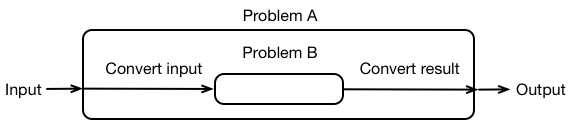
\includegraphics[width=0.6\textwidth]{05_Undecidability/media_upload/reduction.png}
\end{center}
\end{important}


\begin{note}[Turing reductions] \label{note:Turing-reductions}
In the literature, the above idea is formalized using the notion of a \emph{Turing reduction} (with the corresponding symbol $\leq_T$). In order to define it formally, we need to define Turing machines that have access to an \emph{oracle}. This level of detail will not be important for us, so we choose to omit the formal definition in our notes.
\end{note}


\begin{note}[Already established reductions] \label{note:Already-established-reductions}
The proofs of Theorem~\ref{theorem:mathrmACCEPTS-is-undecidable}, Theorem~\ref{theorem:mathrmEMPTY-is-undecidable}, and Theorem~\ref{theorem:mathrmEQ-is-undecidable} correspond to $\text{HALTS} \leq \text{ACCEPTS}$, $\text{ACCEPTS} \leq \text{EMPTY}$ and $\text{EMPTY} \leq \text{EQ}$ respectively.
\end{note}


\begin{flex}
\begin{theorem}[$\mathrm{HALTS} \leq \mathrm{EMPTY}$] \label{theorem:mathrmHALTS-leq-mathrmEMPTY}
$\mathrm{HALTS} \leq \mathrm{EMPTY}$.
\end{theorem}

\begin{proof}
(This can be considered as an alternative proof of Theorem~\ref{theorem:mathrmEMPTY-is-undecidable}.) We want to show that deciding $\text{HALTS}$ reduces to deciding $\text{EMPTY}$. For this, we assume $\text{EMPTY}$ is decidable. Let $M_\text{EMPTY}$ be a decider for $\text{EMPTY}$. We need to construct a TM that decides $\text{HALTS}$. We do so now.

\begin{center}
\includegraphics[width=0.7\textwidth]{05_Undecidability/media_upload/reduction-halts-to-empty.png}
\end{center}

We now argue that this machine indeed decides $\text{HALTS}$. First consider an input $\bkt{M,x}$ such that $\bkt{M,x} \in \text{HALTS}$. Then $L(M') = \Sigma^*$ since in this case $M'$ accepts every string. So when we run $M_\text{EMPTY}(\bkt{M'})$ on line 8, it rejects, and our machine accepts and gives the correct answer. 

Now consider an input $\bkt{M,x}$ such that $\bkt{M,x} \not \in \text{HALTS}$. Then notice that whatever input is given to $M'$, it gets stuck in an infinite loop when it runs $M(x)$. Therefore $L(M')= \emptyset$. So when we run $M_\text{EMPTY}(\bkt{M'})$ on line 8, it accepts, and our machine rejects and gives the correct answer.
\end{proof}
\end{flex}


\begin{flex}
\begin{theorem}[$\mathrm{EMPTY} \leq \mathrm{HALTS}$] \label{theorem:mathrmEMPTY-leq-mathrmHALTS}
$\mathrm{EMPTY} \leq \mathrm{HALTS}$.
\end{theorem}

\begin{proof}
We want to show that deciding $\text{EMPTY}$ reduces to deciding $\text{HALTS}$. For this, we assume $\text{HALTS}$ is decidable. Let $M_\text{HALTS}$ be a decider for $\text{HALTS}$. Using it, we need to construct a decider for $\text{EMPTY}$. We do so now.

\begin{center}
\includegraphics[width=0.7\textwidth]{05_Undecidability/media_upload/reduction-empty-to-halts.png}
\end{center}

We now argue that this machine indeed decides $\text{EMPTY}$. First consider an input $\bkt{M}$ such that $\bkt{M} \in \text{EMPTY}$. Observe that the only way $M'$ halts is if $M(y)$ accepts for some string $y$. This cannot happen since $L(M) = \emptyset$. So $M'(x)$, for \emph{any} $x$, does not halt (note that $M'$ ignores its input). This means that when we run $M_\text{HALTS}(\bkt{M', \epsilon})$, it rejects, and so our decider above accepts, as desired. 

Now consider an input $\bkt{M}$ such that $\bkt{M} \not \in \text{EMPTY}$. This means that there is some word $y$ such that $M(y)$ accepts. Note that $M'$, by construction, does an exhaustive search, so if such a $y$ exists, then $M'$ will eventually find it, and accept. So $M'(x)$ halts for any $x$. When we run $M_\text{HALTS}(\bkt{M', \epsilon})$, it accepts, and our machine rejects and gives the correct answer.
\end{proof}
\end{flex}

%\begin{theorem}
%$\mathrm{HALTS} \leq_T \mathrm{EQ}$.
%\end{theorem}
%\begin{proof}
%This can be considered as an alternative proof of Theorem~\ref{thm:eq}. Assume that $M_\text{EQ}$ is a decider for the language $\text{EQ}$. We construct a TM that decides $\text{HALTS}$ as follows.
%\\\\
%\begin{minipage}[t] \label{theorem:t}{\textwidth}
%\begin{verbatim}
% 1.  "On input <M,x>:
% 2.      Construct the string <M'> where M' is a TM that rejects every input.
% 3.
% 4.      Construct the following string, which we call <M''>.
% 5.      "On input y:
% 6.          run M(x).
% 7.          ignore the output and accept.
% 8.      "
% 9.       
%10.      run M_EQ(<M', M''>).
%11.      if it accepts, reject.
%12.      if it rejects, accept.
%13.  "
%\end{verbatim}
%\end{minipage}
%\\\\
%
%We now argue that this machine indeed decides $\text{HALTS}$. Notice that no matter what the input is, $L(M') = \emptyset$. Let's first consider an input $\bkt{M,x}$ such that $\bkt{M,x} \in \text{HALTS}$. Then $M''$ accepts every input, so $L(M') = \Sigma^*$. In this case, $M_\text{EQ}(\bkt{M',M''})$ rejects, and so our machine accepts as desired. Next, consider an input $\bkt{M,x}$ such that $\bkt{M,x} \not \in \text{HALTS}$. Then whatever input is given to $M''$, it gets stuck in an infinite loop when it runs $M(x)$. So $L(M'')= \emptyset$. In this case $M_\text{EQ}(\bkt{M',M''})$ accepts, and so our machine rejects, as it should. Thus we have a correct decider for $\text{HALTS}$.
%\end{proof}

%\begin{exercise} \label{ex:reduction-properties} \
%\begin{enumerate}
%    \item[(a)] \label{exercise:a} Let $A$, $B$ and $C$ be languages. Show that if $A \leq_T B$ and $B \leq_T C$, then $A \leq_T C$.
%    \item[(b)] Give a counter-example for the following claim: if $A \leq_T B$ then $B \leq_T A$.
%\end{enumerate}
%\end{exercise}

\begin{flex}
\begin{exercise}[Practice with reduction definition] \label{exercise:Practice-with-reduction-definition}
Let $A, B \subseteq \{\s{0},\s{1}\}^*$ be languages. Prove or disprove the following claims.
\begin{enumerate}
    \item[(a)] If $A \leq B$ then $B \leq A$.
    \item[(b)] If $A \leq B$ and $B$ is regular, then $A$ is regular. 
\end{enumerate}
\end{exercise}

\begin{solution}
Part 1: The claim is false. Let $A$ be any decidable language. For example, we can take $A = \emptyset$. The decider for $A$ is a machine that rejects no matter what the input is. Let $B = \text{HALTS}$. Then to establish $A \leq B$, we need to argue that given a decider for $\text{HALTS}$, we can decide $\emptyset$. Since $\emptyset$ is decidable, this is true (and we don't even need to make use of a decider for $\text{HALTS}$). On the other hand, it is \textbf{not} true that $\text{HALTS} \leq \emptyset$. For the sake of contradiction, if it was true, then this would mean that using a decider for $\emptyset$, we can decide $\text{HALTS}$. And this would imply that $\text{HALTS}$ is decidable, a contradiction.
\\\\
\noindent
Part 2: The claim is false. Consider $A = \{0^n1^n: n \in \N\}$ and $B = \emptyset$. We have $A \leq B$ because $A$ is a decidable language (we don't even need to make use of the decider for $B$). Furthermore, $B$ is regular, but $A$ is not.
\end{solution}
\end{flex}


\begin{flex}
\begin{exercise}[Practice with reduction proofs] \label{exercise:Practice-with-reduction-proofs}
Show the following.
\begin{enumerate}
    \item[(a)] $\text{ACCEPTS} \leq \text{HALTS}$.
    \item[(b)] $\text{HALTS} \leq \text{EQ}$.
\end{enumerate}
\end{exercise}

\begin{solution}
Part 1: We want to show that $\text{ACCEPTS}$ reduces to $\text{HALTS}$. To do this, we assume that $\text{HALTS}$ is decidable. Let $M_\text{HALTS}$ be a decider for $\text{HALTS}$. We now need to construct a TM that decides $\text{ACCEPTS}$ (which will make use of $M_\text{HALTS}$). Here is the description of the decider:

\begin{center}
\includegraphics[width=0.7\textwidth]{05_Undecidability/media_upload/reduction-accepts-to-halts.png}
\end{center}

We now argue that this machine indeed decides $\text{ACCEPTS}$. Note that given $\bkt{M,x}$, there are three possibilities: $M(x)$ accepts; $M(x)$ rejects, $M(x)$ loops. And $\bkt{M,x} \in \text{ACCEPTS}$ if and only if $M(x)$ accepts. 

Let's first consider an input $\bkt{M,x}$ such that $\bkt{M,x} \in \text{ACCEPTS}$. Then $M_\text{HALTS}(\bkt{M,x})$ must accept, i.e. $M(x)$ halts. So the decider above safely simulates $M(x)$ on line 4 and accepts (on line 5).

If the the input is such that $\bkt{M,x} \not \in \text{ACCEPTS}$, then there are two cases. Either $M(x)$ halts but rejects, or $M(x)$ loops. If it is the latter, then $M_\text{HALTS}(\bkt{M,x})$ rejects, and therefore our decider rejects as well. If on the other hand $M(x)$ halts but rejects, then our decider safely simulates $M(x)$ on line 4 and rejects (on line 6).

Whatever the input is, our decider gives the correct answer. The proof is complete.
\\\\
\noindent
Part 2: (This can be considered as an alternative proof of Theorem~\ref{theorem:mathrmEQ-is-undecidable}.) We want to show that $\text{HALTS}$ reduces to $\text{EQ}$. To do this, we assume that $\text{EQ}$ is decidable. Let $M_\text{EQ}$ be a decider for $\text{EQ}$. We now need to construct a TM that decides $\text{HALTS}$ (which will make use of $M_\text{EQ}$). Here is the description of the decider:

\begin{center}
\includegraphics[width=0.7\textwidth]{05_Undecidability/media_upload/reduction-halts-to-eq.png}
\end{center}

We now argue that this machine indeed decides $\text{HALTS}$. Notice that no matter what the input is, $L(M') = \emptyset$. Let's first consider an input $\bkt{M,x}$ such that $\bkt{M,x} \in \text{HALTS}$. Then $M''$ accepts every input, so $L(M') = \Sigma^*$. In this case, $M_\text{EQ}(\bkt{M',M''})$ rejects, and so our machine accepts as desired. Next, consider an input $\bkt{M,x}$ such that $\bkt{M,x} \not \in \text{HALTS}$. Then whatever input is given to $M''$, it gets stuck in an infinite loop when it runs $M(x)$. So $L(M'')= \emptyset$. In this case $M_\text{EQ}(\bkt{M',M''})$ accepts, and so our machine rejects, as it should. Thus we have a correct decider for $\text{HALTS}$.
\end{solution}
\end{flex}



%%%%%%%%%%%%%%%%%%%%%%%%%%%%%%%%%%
%%%%%%%%%%%%%%%%%%%%%%%%%%%%%%%%%%
%%%%%%%%%%%%%%%%%%%%%%%%%%%%%%%%%%


\section{Check Your Understanding}

\begin{enumerate}
    \item True or false: For languages $K$ and $L$, if $K \leq L$, then $L$ is undecidable.
    \item True or false: For languages $K$ and $L$, if $K \leq L$ and $L \leq K$, then $L$ and $K$ are both decidable.
    \item True or false: Fix an alphabet $\Sigma$. The set of undecidable languages is countable.
    \item True or false: Fix an alphabet $\Sigma$. The set of decidable languages is infinite.
    \item True or false: If languages $K$ and $L$ are both undecidable, then their union is also undecidable.
    \item True or false: If a language $L$ is undecidable, then $L$ is infinite.
    \item True or false: $\Sigma^* \leq \emptyset$.
    \item True or false: $\text{HALTS} \leq \Sigma^*$.
    \item True or false: Every decidable language reduces to $\text{HALTS}$. 
    \item True or false: All unary languages (i.e. languages over the alphabet $\Sigma = \{1\}$) are decidable.
\end{enumerate}



%%%%%%%%%%%%%%%%%%%%%%%%%%%%%%%%%%%%%%%%%%%%%
%%%%%%%%%%%%%%%%%%%%%%%%%%%%%%%%%%%%%%%%%%%%%
%%%%%%%%%%%%%%%%%%%%%%%%%%%%%%%%%%%%%%%%%%%%%

\section{Mastery List}

\begin{enumerate}
    \item You should be able to easily argue the existence of undecidable languages by a counting argument: The set of all languages is uncountable whereas the set of decidable languages is countable. This shows that almost all languages are undecidable, however, it does not give us an explicit undecidable language.
    \item Turing's theorem establishes an explicit language that is undecidable. You should be able to explain this proof to someone else without looking at your notes.
    \item You should be comfortable with the concept of a reduction. We have seen in an earlier chapter that reductions can be used to expand the landscape of decidable languages. In this chapter, you see that it can be used to expand the landscape of undecidable languages. Make sure you understand why this is the case.
    \item You should be comfortable with undecidability proofs. This chapter has many examples of such proofs. It is easy to fall in the trap of trying to memorize the template of such proofs rather than really understanding the logic behind how and why these proofs work. Don't fall in this trap. Each step of the argument should make perfect sense. If you struggle to understand these proofs, it is usually a sign that there are gaps in your knowledge from previous chapters. Come talk to us so we can help you identify those gaps.
\end{enumerate}
